\documentclass{report}

\usepackage[vietnamese]{babel}
\usepackage{vntex}
\usepackage{hyperref}
\usepackage{fancyhdr}
\usepackage{etoc}
\usepackage{tgschola}
\usepackage{minted}
\usepackage{graphicx}
\graphicspath{{./img/}}
\usepackage{titlesec}
\usepackage{titletoc}
\usepackage{algpseudocode}
\usepackage[a5paper,left=20mm,right=20mm,bottom=20mm,top=20mm]{geometry}
\usepackage{multicol}

\newtheorem{theorem}{Định lý}

\title{Sổ tay Cấu trúc Dữ liệu và Giải thuật}
\author{Một sinh viên K23 ngành Khoa học Máy tính \\ (CT Định hướng Nhật Bản) \\ Trường ĐH Bách khoa, ĐHQG-HCM}
\date{\today}

\hypersetup{
    colorlinks,
    citecolor=black,
    filecolor=black,
    linkcolor=black,
    urlcolor=blue
}

\pagestyle{fancy}
\lhead{}
\rhead{Sổ tay Cấu trúc Dữ liệu và Giải thuật}

\begin{document}

\maketitle

\chapter*{Lời nói đầu}
Tuy gọi là chuyên đề về "Cấu trúc dữ liệu và giải thuật" nhưng thực ra, ta mới chỉ tìm hiểu về một số cấu trúc dữ liệu và giải thuật hay gặp. Không một tài liệu nào có thể đề cập tới mọi cấu trúc dữ liệu và giải thuật bởi chúng quá phong phú và liên tục được bổ sung. Việc đi sâu nghiên cứu những cấu trúc dữ liệu và giải thuật, dù chỉ là một phần nhỏ hẹp cũng nảy sinh rất nhiều vấn đề hay và khó, như các vấn đề lý thuyết về độ phức tạp tính toán, vấn đề NP-đầy đủ v.v… Đó là công việc của những nhà khoa học máy tính. Nhưng trước khi trở thành một nhà khoa học máy tính thì điều kiện cần là phải biết lập trình. Vậy nên khi tìm hiểu bất cứ cấu trúc dữ liệu hay giải thuật nào, nhất thiết ta phải cố gắng cài đặt bằng được. Mọi ý tưởng hay sẽ chỉ là bỏ đi nếu như không biến thành hiệu quả, thực tế là như vậy.

Tôi xin cảm ơn \href{https://wiki.vnoi.info}{VNOI Wiki} và cuốn sách "Giải thuật và Lập trình" của thầy Lê Minh Hoàng đã là nguồn tư liệu tham khảo quý giá giúp tôi hoàn thành tài liệu này.

\tableofcontents
\thispagestyle{empty} % remove page number on ToC

\renewcommand{\contentsname}{}

\titleformat{\chapter}[block]%
{\bfseries\Large\filleft}%
{\fontsize{60}{50}\selectfont\color{gray}\thechapter}%
{1em}
{\fontsize{30}{50}\selectfont\scshape}%
[\vspace{-2ex}\normalsize\normalfont\vspace*{1cm}%
\hbox{\large\bfseries\contentsname}\vspace{0.5cm}\titlerule\vspace{0.5cm}
\startcontents
\printcontents{l}{1}{\setcounter{tocdepth}{1}}\vspace{0.5cm}
\titlerule\vspace{1pc}]

\chapter{Giải thuật quay lui}
\section{Giới thiệu}
Dùng để giải bài toán liệt kê cấu hình. Mỗi cấu hình được xây dựng bằng cách chọn từng phần tử, mỗi phần tử được chọn bằng cách thử tất cả các khả năng theo quy tắc nhân.

Mã giả cho thuật toán quay lui:
\begin{algorithmic}
    \State $x\gets[]$
    \Comment{Khai báo mảng $x$ lưu cấu hình hiện tại}
    \Function{Try}{$i$}
        \Comment{Thử cho phần tử $x_i$}
        \For{$j$ trong tập giá trị cho $x_i$}
            \State $x_i\gets j$
            \If{$i=n$}
                \Comment{$n$ là số phần tử của cấu hình}
                \State{Thông báo cấu hình trong $x$}
            \Else
                \State{<Thời điểm cuối cùng để ghi nhận kết quả>}
                \State\Call{Try}{i+1}
                \State{<Bỏ ghi nhận giá trị $x_i\gets j$ để thử giá trị khác>}
            \EndIf
        \EndFor
    \EndFunction
\end{algorithmic}

Thuật toán quay lui sẽ bắt đầu bằng lời gọi \texttt{Try(0)}, \texttt{Try(1)} hoặc với chỉ số mảng x mà ta muốn bắt đầu xây dựng.

Vì thuật toán này rất dễ nên tất cả các ví dụ trong bài này sẽ do người đọc tự làm.

\section{Liệt kê dãy nhị phân độ dài n}
Dùng mảng x để lưu dãy nhị phân hiện tại. Biết rằng $j\in\{0,1\}$.
\begin{figure}[h]
    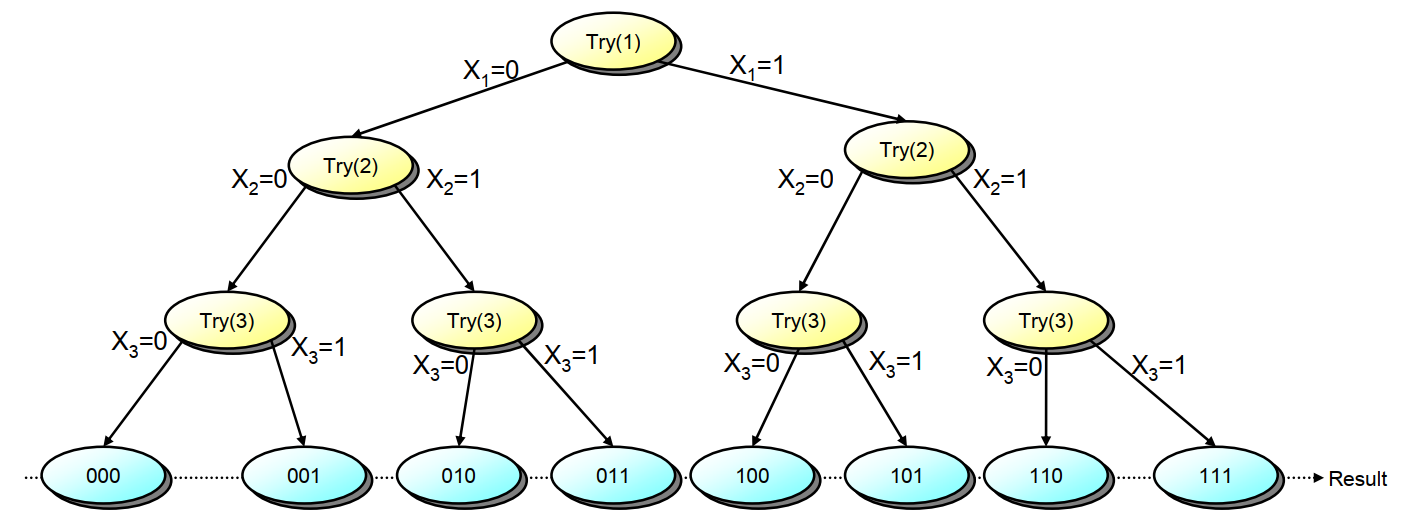
\includegraphics[scale=0.3]{quaylui/lknp.png}
    \caption{Cây tìm kiếm quay lui với n = 3}
\end{figure}

\section{Liệt kê các tổ hợp chập k}
Đây là bài toán biến thể của bài toán trên, với $j$ thuộc tập các phần tử (nếu nó chưa được chọn).

\section{Bài toán phân tích số}
Cho một số $n\leq30$, hãy liệt kê tất cả các cách phân tích nó thành một tổng.

\begin{tabular}{l|l}
    ANALYSE.INP & ANALYSE.OUT\cr\hline
    6 & 6 = 1 + 1 + 1 + 1 + 1 + 1\cr
      & 6 = 1 + 1 + 1 + 1 + 2\cr
      & 6 = 1 + 1 + 1 + 3\cr
      & 6 = 1 + 1 + 2 + 2\cr
      & 6 = 1 + 1 + 4\cr
      & 6 = 1 + 2 + 3\cr
      & 6 = 1 + 5\cr
      & 6 = 2 + 2 + 2\cr
      & 6 = 2 + 4\cr
      & 6 = 3 + 3\cr
      & 6 = 6\cr
\end{tabular}

Đây là bài toán biến thể của bài toán trên, với $j\in[1;n]$. Để cho thuận tiện ta dùng thêm mảng t với $t_i$ là tổng các phần tử từ $x_1\dots x_i$. Lưu ý:
\begin{itemize}
    \item Để tránh trùng lặp (hoán vị) ta sẽ đặt thêm điều kiện $x_i\geq x_{i-1}$.
    \item Để đặt điều kiện dừng (vì lần này ta không có số phần tử cố định) đồng thời tăng tốc độ cho đệ quy (không xét những giá trị thừa), ta chọn $x_i$ sao cho $t_{i+1}\leq n$ hay
    $$
        t_{i+1}\leq n\Leftrightarrow t_{i-1}+x_i+x_{i+1}\leq n\Leftrightarrow x_i+x_{i+1}\leq n-t_{i-1}
    $$
    mà $x_{i+1}\geq x_i$ nên suy ra $x_i\leq(n-t_{i-1})/2$. Ví dụ khi $n=10$ mà chọn $x_0\in\{6,7,8,9,10\}$ thì ta không thể chọn tiếp $x_1$, vậy chọn $x_0$ như vậy vô nghĩa.

    \textbf{Tóm lại: ta gọi đệ quy tìm tiếp khi $x_i$ được chọn còn cho phép chọn $x_{i+1}\geq x_i$ mà không làm tổng vượt quá n, ta in kết quả ở lần đệ quy cuối khi $t_i=n$.}
\end{itemize}

\section{Bài toán xếp hậu}
Cho bàn cờ vua n x n. Tìm cách xếp n quân hậu trên bàn cờ sao cho không quân nào ăn được quân nào.

Ví dụ n = 8:

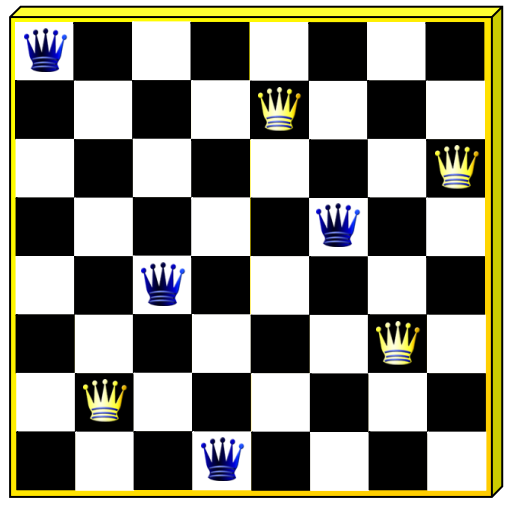
\includegraphics[scale=0.5]{quaylui/xephau.png}

Rõ ràng n quân hậu sẽ được đặt mỗi con 1 hàng vì hậu ăn ngang được, mỗi con 1 cột vì hậu cũng ăn dọc được, vậy nếu gọi quân hậu i là quân hậu ở hàng i, ta chỉ cần tìm ra vị trí cột của từng quân là sẽ giải được một nghiệm của bài toán. Có một tính chất dễ nhận thấy nếu ta làm các bài toán liên quan đến bảng nhiều:
\begin{itemize}
    \item Ta dùng mảng a để đánh dấu xem cột đó có con hậu nào chưa. ($a_i$ = true nếu đã có và ngược lại).
    \item Mọi đường chéo hướng ĐB-TN đều có các ô với số hàng + số cột là một hằng số C. 8 đường chéo có tổng lần lượt là 2, 4, \dots 2n. Vậy ta có thể dùng mảng b kích cỡ 2n với $a_C$ = true biểu thị đường chéo ĐB-TN chưa có quân hậu nào kiểm soát và ngược lại.
    \item Mọi đường chéo hướng ĐN-TB đều có các ô với số hàng - số cột là một hằng số C. Làm tương tự như trên với mảng c.
\end{itemize}

Vậy ta xây dựng thuật toán quay lui: Đặt từng quân hậu, đánh dấu trên các mảng a, b, c và gọi đệ quy đặt quân tiếp theo với điều kiện đã nêu $(a_j = b_{i+j} = c_{i-j}$ = true).
\chapter{Bài toán tìm kiếm}
\section{Giới thiệu}
Bài toán tìm kiếm là một trong những vấn đề thường gặp nhất trong cuộc sống, và kể cả trong máy tính. Tìm một cuốn sách trên tủ sách, tìm chương mà mình yêu thích trong cuốn sách, tìm loại nội dung đang tìm trong đó\dots. Thật vô vàn ví dụ thực tế. Ở đây mình sẽ trình bày những thuật toán tìm kiếm cơ bản trong tìm kiếm dữ liệu trên máy tính.

Đối với các CTDL cây, mình sẽ không trình bày cách thêm, xoá nút cho cây, các bạn tự tìm hiểu nhé.

\section{Tìm kiếm tuần tự}
Phát biểu bài toán: Cho dãy số S. Tìm vị trí giá trị $x$ trong dãy.

Đơn giản là dùng một vòng lặp duy nhất duyệt toàn bộ S, nếu trong quá trình duyệt ta tìm được giá trị $S_i=x$ thì dừng / tìm tiếp tuỳ theo yêu cầu bài toán và thông báo kết quả. Dễ nhận thấy rằng độ phức tạp tính toán trung bình của thuật toán này là $O(n)$. Với n rất lớn, thuật toán này sẽ thất bại.

\section{Tìm kiếm nhị phân}
Bình thường khi tìm một con số trên một dãy số tăng dần / giảm dần, bạn sẽ tìm từ trái sang phải, phải sang trái hay đoán vị trí mà giá trị cần tìm có thể ở đó và chỉ tìm kiếm tại khu vực đó? Thuật toán tìm kiếm nhị phân được xây dựng trên tư tưởng thứ hai, và vì vậy, nó chỉ hoạt động nếu danh sách đã được sắp xếp, nếu không, không còn cách nào khác ngoài tìm kiếm tuần tự như trong thực tế.

Giả sử $S=\{S_1,S_2,\dots,S_n\}$.

Ta sẽ tìm kiếm trên đoạn [l, r] với l = 1, r = n. Thuật toán lặp lại với việc kiểm tra giá trị giữa đoạn. Ta sẽ kiểm tra $S_{n/2}$ có bằng x không:
\begin{itemize}
    \item Nếu $S_{n/2}=x$, trả về giá trị $n/2$. Thuật toán kết thúc.
    \item Nếu $S_{n/2}>x$, vậy x phải nằm ở nửa bên trái của mảng, ta lặp lại thuật toán với nửa mảng con trái bằng cách đặt $r=m-1$.
    \item Nếu $S_{n/2}<x$, tương tự ta đặt $l=m+1$.
\end{itemize}

Cách cài đặt vừa được mô tả ở trên là cách cài đặt tuyến tính dùng một vòng lặp while. Có thể được cài đặt bằng đệ quy, nhưng vì tốc độ của đệ quy chậm hơn vòng lặp nên mình ưu tiên cài đặt theo cách đầu tiên.

Về độ phức tạp, dễ thấy rằng sau mỗi lần lặp độ dài dãy giảm đi 1 nửa, vậy chỉ mất $\log_2n$ thao tác thì độ dài mảng chỉ còn 1, ta chỉ việc kiểm tra xem nó có phải x không. Vậy độ phức tạp thời gian của nó là $O(\log_2n)$.

\section{Cây tìm kiếm nhị phân (Binary Search Tree - BST)}
Bản chất của cây là tìm kiếm nhị phân, tuy nhiên với tìm kiếm nhị phân ta phải sắp xếp dãy số rồi mới áp dụng được, đối với cây tìm kiếm nhị phân trong quá trình ta nhập dãy ta sẽ xây dựng cây luôn, sau đó tìm giá trị thông qua các nhánh của nó.

Cây là một cây nhị phân cân bằng, với mỗi nút, nút con trái chứa giá trị nhỏ hơn nó và nút con phải chứa giá trị lớn hơn nó. Vậy nếu đi theo nhánh trái đến cuối cây ta sẽ gặp giá trị nhỏ nhất và đi theo nhánh phải đến cuôi cây ta sẽ gặp giá trị lớn nhất.

Ví dụ với dãy S = [4, 7, 3, 5, 2, 6, 1]. Ta xây được cây như sau:

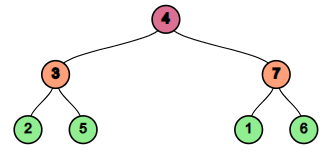
\includegraphics{timkiem/caynpmau.png}

Nguyên tắc xây cây: xây từ trên xuống dưới, từ trái qua phải để đảm bảo tính cân bằng của cây. Dễ nhận thấy nhược điểm rằng thuật toán hoạt động chậm khi cây bị suy biến (cây trở thành một đường thẳng nếu dãy đã được sắp xếp sẵn), lúc này mọi thao tác đều có độ phức tạp tính toán $O(n)$, lúc này người ta sẽ sử dụng cây nhị phân tìm kiếm tối ưu, hoặc dựng cây nhị phân tự cân bằng AVL.

Việc xây cây này cũng là một dạng sắp xếp (người ta gọi phương pháp này là Tree Sort), ta có thể đi theo các nhánh của nó tuỳ vào quan hệ của nó với nút ta đang xét đến khi tìm ra giá trị cần tìm. Và vì chiều cao của cây là $\log_2n$, độ phức tạp \textbf{trung bình} của thuật toán cũng là $O(\log_2n)$. Thời gian xây cây từ một dãy là $O(n)$ và thời gian vừa xây vừa nhập là $O(n\log_2n)$, tương đương với các thuật toán sắp xếp (vì phải đi dọc theo cây để chèn).

\section{Cây tìm kiếm số học (Digital Search Tree - DST)}
Là một cây nhị phân tìm kiếm, nhưng nút con trái của mỗi nút tại mức k của cây sẽ chứa giá trị có bit k là 0, nút con phải sẽ chứa giá trị có bit k là 1. Và vì hiển nhiên giá trị nút con phải lớn hơn cây con trái $2^k$ đơn vị, điều này giống với cây nhị phân tìm kiếm, nhưng lúc này thao tác tìm kiếm trên cây chỉ còn là $O(\log_2\max\{S_i\})$.

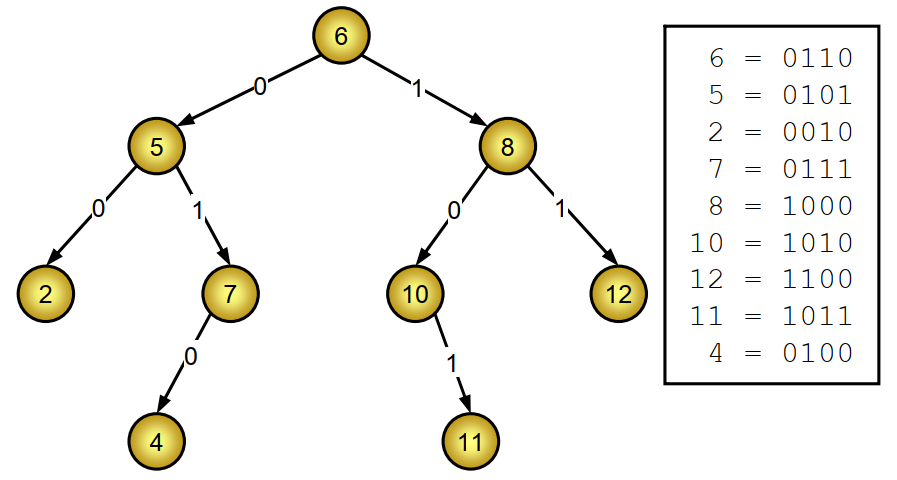
\includegraphics[scale=0.45]{timkiem/caytksohoc.png}

\section{Cây tìm kiếm cơ số (Radix Search Tree - RST)}
Là một cây tìm kiếm số học, nhưng giá trị của dãy chỉ nằm ở các nút lá, còn giá trị trong các nút còn lại là vô nghĩa. Quy ước vẫn giữ nguyên như cây tìm kiếm số học, ta đi theo các nhánh sẽ đến được giá trị cần tìm, nếu không có nút nào ở đó thì tìm kiếm thất bại.

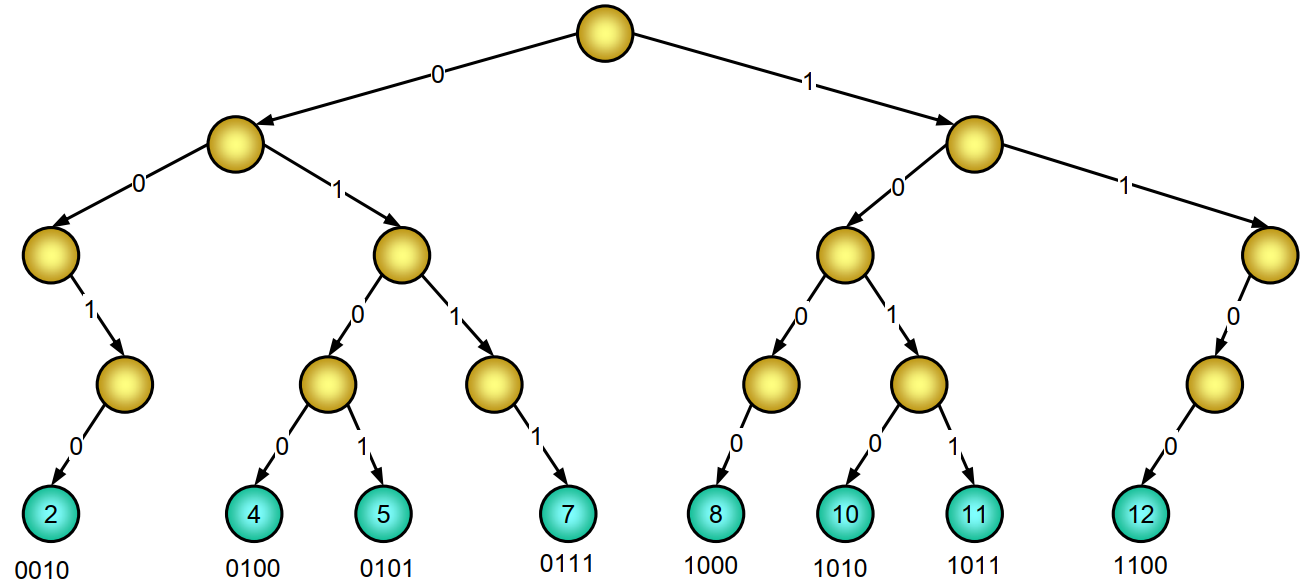
\includegraphics[scale=0.3]{timkiem/caytkcoso2.png}

Các cây tìm kiếm ở trên còn có một nhược điểm: nếu quá trình so sánh giá trị trong khi duyệt phức tạp và mất nhiều thời gian, chúng sẽ hoạt động chậm. RST đã khắc phục được nhược điểm này, nhưng lại có một nhược điểm mới là tốn rất nhiều bộ nhớ vì các giá trị vô nghĩa, ngoài ra để tăng tốc độ tìm kiếm ta có thể dùng cây k-phân thay vì nhị phân nhưng độ phức tạp bộ nhớ sẽ tăng lên.
\chapter{Bài toán sắp xếp}
Khi so sánh các thuật toán sắp xếp, ta quan tâm tới một số điều:
\begin{itemize}
    \item \textbf{Thời gian chạy}: với lượng dữ liệu lớn máy sẽ mất rất nhiều thời gian để chạy, không thể sử dụng trong thực tế.
    \item \textbf{Bộ nhớ}: đối với các hệ thống bộ nhớ thấp (hệ thống nhúng), một vài thuật toán sẽ không thể chạy được.
    \item \textbf{Tính ổn định}: Đối với thuật toán sắp xếp ổn định, các phần tử có giá trị bằng nhau sẽ giữ nguyên thứ tự như trước khi sắp xếp. Tính ổn định có vai trò quan trọng khi ta sắp xếp nhiều lần để tuân theo nhiều tiêu chí.
\end{itemize}
Trong khuôn khổ chương này, chỉ có thuật toán Bubble Sort, Insertion Sort và Merge Sort là ổn định. Về minh hoạ, trừ Heap Sort ra bạn đều có thể đến \href{https://visualgo.net/en/sorting}{VisualAlgo}.

\section{Thuật toán Bubble Sort}
Cho dãy S với n phần tử cần được sắp xếp tăng dần. Xét các phần tử $a_i$ và $a_{i+1}$. Nếu $a_i>a_{i+1}$, ta đổi chỗ hai phần tử. Nói cách khác, phần tử nhỏ nhất sẽ \textbf{nổi} lên trên, vì vậy đây còn được gọi là thuật toán sắp xếp nổi bọt. Lặp lại đến khi không còn 2 phần tử nào thoả mãn.

\begin{minted}{cpp}
for (int i = 0; i < n; i++)
    for (int j = 0; j < n - 1; j++)
        if (a[j] > a[j + 1])
            swap(a[j], a[j + 1]);
\end{minted}

Dễ thấy rằng sau mỗi vòng lặp của i, các phần tử cần được sắp xếp sẽ được dịch chuyển 1 vị trí. Vậy trong trường hợp xấu nhất (phần tử lớn nhất nằm ở đầu dãy hoặc phần tử nhỏ nhất ở cuối dãy), cả n vòng lặp i đều sẽ được dùng để đưa phần tử này về đúng vị trí. Các trường hợp còn lại sẽ không dùng tới toàn bộ n vòng lặp, nhưng để đảm bảo, ta lặp đến n cho i. Vậy độ phức tạp thời gian là $O(n^2)$, độ phức tạp bộ nhớ là $O(1)$.
\section{Thuật toán Insertion Sort}
Ý tưởng của thuật toán này là sẽ đưa từng phần tử một về đúng vị trí của nó trong dãy. Giả sử dãy đã có i phần tử được sắp xếp, ta tìm chỗ cho phần tử thứ i + 1 và \textbf{chèn} nó vào đó. Vì vậy đây còn được gọi là thuật toán sắp xếp chèn.

Ta thấy rằng khi dãy đã gần được sắp xếp xong, Insertion Sort sẽ chạy rất nhanh, ví dụ như sắp xếp điểm cao trong game.

\begin{minted}{cpp}
for (int i = 1; i < N; i++) {
    // Tìm vị trí phù hợp cho S[i] bằng tìm kiếm nhị phân
    int l = 0, r = i - 1;
    while (l <= r) {
        int m = (l + r) / 2;
        if (S[m] < S[i])
            l = m + 1;
        else
            r = m - 1;
    }
    // Đưa S[i] về vị trí l (dời dãy)
    int tmp = S[i];
    for (int k = i; k > l; k--)
        S[k] = S[k - 1];
    S[l] = tmp;
}
\end{minted}

Đánh giá về độ phức tạp, dễ thấy rằng ta cần 1 vòng lặp để duyệt qua mọi phần tử, và 1 vòng lặp nữa để đưa nó về đúng vị trí (ta chỉ quan tâm đến độ phức tạp lớn nhất trong vòng lặp, trong trường hợp này là $O(n)$). Trong trường hợp xấu nhất như Bubble Sort, vòng lặp này sẽ có độ phức tạp $O(n)$. Vậy độ phức tạp thời gian là $O(n)$, độ phức tạp bộ nhớ là $O(1)$.

\section{Thuật toán Shell Sort - Insertion Sort cải tiến}
Nhược điểm của Insertion Sort là sẽ mất rất nhiều thao tác để ta có thể chèn phần tử vào vị trí gần đầu dãy. Shell Sort tối ưu hoá theo tư tưởng chia dãy số thành nhiều dãy con, với dãy con $S_1=\{S_0,S_{h},S_{2h}\dots\},S_2=\{S_1,S_{1+h},S_{1+2h}\dots\}\dots$ với h là bước, ta có thể chọn h sao cho phù hợp. Ví dụ với dãy (4, 6, 7, 2, 3, 5, 1, 9, 8), h = 3:

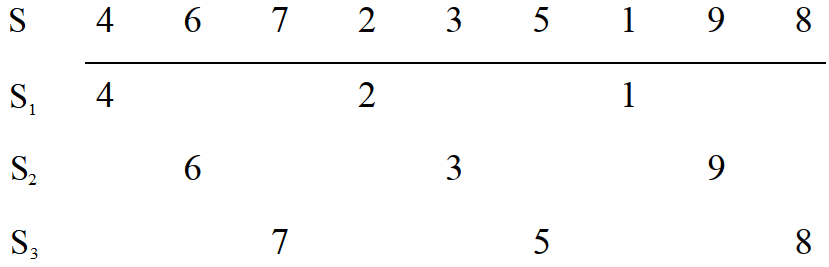
\includegraphics[scale=0.45]{sapxep/shellsort.png}

Dễ thấy rằng ở thao tác dời dãy, phần tử $S_6=1$ thay vì phải thao tác trên 6 phần tử trước nó thì giờ đây chỉ cần thao tác qua 2 phần tử, nhanh chóng được đưa về vị trí \textbf{gần đúng} của nó. Để tăng độ chính xác (tìm vị trí chính xác), ta chia đôi h đến khi h = 1 (có nghĩa là gộp 2 dãy con lại), ta được dãy sắp xếp.

\section{Thuật toán Heap Sort}
Trong khuôn khổ này, heap đơn giản là một cây nhị phân với nút cha mang giá trị lớn hơn 2 nút con.

Nếu vậy, nút gốc sẽ mang giá trị lớn nhất trong dãy. Vậy ta sẽ lấy giá trị nút gốc cho vào cuối dãy, sau đó xoá nút gốc đi, đưa nút lá cuối cùng lên gốc, lúc này heap không còn đúng nữa, ta sẽ đảo các nút sao cho đúng thứ tự trở lại, việc này gọi là \textbf{vun đống heap}, vì vậy đây còn được gọi là thuật toán sắp xếp vun đống. Lặp lại đến khi heap rỗng.

Khi sắp xếp tăng dần, ta thu được một cây, trong đó nút gốc là phần tử lớn nhất của dãy, hay còn gọi là \textbf{max heap}, ngược lại với \textbf{min heap}.

Ví dụ với dãy S = [4, 7, 3, 5, 2, 6, 1]. Hình bên trái là cây nhị phân sau khi xây, bên phải là sau khi được vun đống.

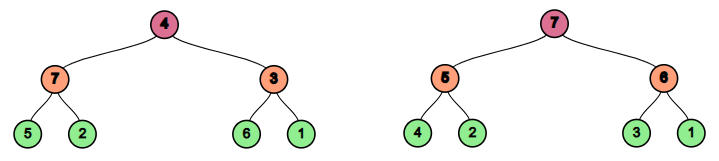
\includegraphics[scale=0.55]{sapxep/heapify}

Độ phức tạp thời gian là $O(n\log_2n)$ vì ta phải vun đống $n$ lần, vì vun đống duyệt theo chiều cao của cây, tối đa là $\log_2n$. Độ phức tạp bộ nhớ là $O(1)$.

\section{Thuật toán Quick Sort}
Ta chia dãy thành 2 phần, một phần "lớn" và một phần "nhỏ" bằng cách chọn một phần tử chốt (hay gọi là \textbf{pivot}), đưa nó về đúng vị trí bằng Insertion Sort, tiếp tục gọi đệ quy cho từng phần đến khi mỗi phần chỉ còn 2 phần tử (điều kiện dừng đệ quy) và sắp xếp 2 phần tử.

Thuật toán này nổi tiếng vì nó chạy nhanh nhất trong tất cả các thuật toán sắp xếp dựa theo so sánh (tác giả của nó đã tự tin đặt cho nó cái tên Quick Sort - sắp xếp nhanh), được sử dụng nhiều trong các thư viện của Java, C++ (hàm \texttt{sort} của C++ dùng Intro Sort là kết hợp giữa Quick Sort và Insertion Sort).

Tuy nhiên, ta thấy rằng độ phức tạp thời gian có phần ngẫu nhiên, phụ thuộc vào cách chọn \textbf{pivot}, nếu tất cả pivot được chọn đều trong trường hợp xấu nhất như trên, độ phức tạp sẽ tương đương với Insertion Sort $O(n^2)$, nhưng trong trường hợp ngẫu nhiên, trung bình là $O(n\log_2n)$ (ta chia đôi dãy sau mỗi lần gọi đệ quy, vậy có tối đa $\log_2n$ lần chia).

\begin{minted}{cpp}
void quickSort(int* S, int l, int r) {
    // điều kiện dừng đệ quy
    if (l >= r) return;
    
    int i = l, j = r;
    int pivot = S[l + rand() % (r - l + 1)];

    // đưa pivot về đúng vị trí
    while (i <= j) {
        while (S[i] < pivot) i++;
        while (S[j] > pivot) j--;
        if (i <= j) {
            std::swap(S[i], S[j]);
            i++; j--;
        }
    }

    // gọi đệ quy sắp xếp phần bên trái
    quickSort(S, l, j);
    // gọi đệ quy sắp xếp phần bên phải
    quickSort(S, i, r);
}
\end{minted}

Phân tích về chọn ngẫu nhiên pivot, một số ví dụ sau đây sẽ làm Quick Sort bị suy biến:
\begin{itemize}
    \item pivot = $S_0$ (phần tử đầu tiên) hoặc pivot = $S_n$ (phần tử cuối cùng) thì dễ thấy rằng nó sẽ gọi đệ quy cho phần bên phải/trái liên tục $n$ lần, gây ra độ phức tạp $O(n^2)$.
    \item pivot = $S_m$ (phần tử giữa), với m lớn thì nó cũng bị suy biến.
\end{itemize}
Vậy cách tốt nhất là chọn ngẫu nhiên để trung bình hoá các lần chọn tốt và lần chọn không tốt nhằm chạy với độ phức tạp trung bình.

\section{Thuật toán Merge Sort}
Thuật toán sắp xếp đệ quy này chia đôi dãy số, so sánh hai phần tử của nó và trộn lại nên được gọi là thuật toán \textbf{sắp xếp trộn}.

Đầu tiên ta tạo một mảng S' khác để lưu mảng đã sắp xếp.

Ta chia đôi dãy số (gọi đệ quy đến khi dãy con chỉ còn 1 phần tử), so sánh hai phần tử đầu tiên của hai phần. Phần tử nhỏ hơn ta cho vào S' và xoá khỏi phần tương ứng. Tiếp tục so sánh bằng vòng lặp đến khi đã cho hết hai dãy vào S', Sao chép dữ liệu trở lại dãy S và lặp lại đến khi sắp xếp xong.

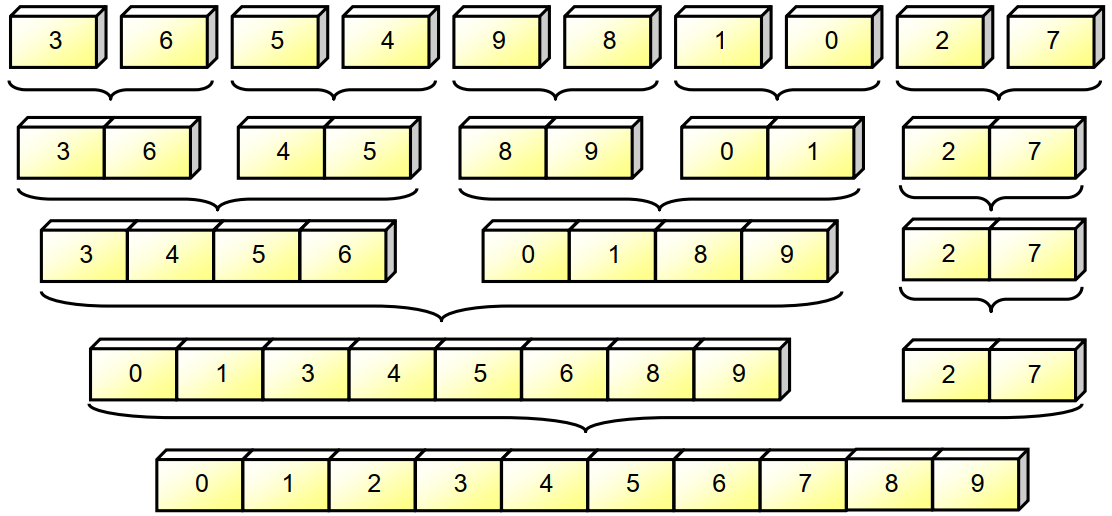
\includegraphics[scale=0.35]{sapxep/mergesort.png}

Độ phức tạp thời gian tương tự như Quick Sort $O(n\log_2n)$ nhưng độ phức tạp bộ nhớ là $O(n)$ do mảng S'.

\begin{minted}{cpp}
// giả sử N là số phần tử
int S_[N]; // S'

void mergeSort(int* S, int l, int r) {
    // dãy chỉ gồm 1 phần tử, điều kiện dừng đệ quy
    if (l >= r) return;
    // chia đôi dãy
    int m = l + (r - l) / 2;
    // gọi đệ quy chia đôi
    mergeSort(S, l, m);
    mergeSort(S, m + 1, r);
    // bắt đầu so sánh
    int i = l, j = m + 1;
    int cur = 0; // vị trí phần tử trong S'
    while (i <= m || j <= r) {
        // bên trái không còn phần tử nào
        if (i > m)
            S_[cur++] = S[j++];
        // bên phải không còn phần tử nào
        else if (j > r)
            S_[cur++] = S[i++];
        // phần tử bên trái nhỏ hơn
        else if (S[i] < S[j])
            S_[cur++] = S[i++];
        else
            S_[cur++] = S[j++];
    }
    // copy mảng S_ trở lại S
    for (int k = 0; k < cur; k++)
        S[l + k] = S_[k];
}
\end{minted}

\section{Thuật toán Radix Sort}
Thuật toán này đặc biệt hơn các thuật toán khác ở chỗ, nó không sắp xếp theo so sánh số, nhưng sắp xếp theo so sánh chữ số của các số đó, nên được gọi là thuật toán so sánh \textbf{theo cơ số}.

Ta chia các phần tử theo các nhóm (dựa theo bit đầu tiên, chữ số đầu tiên\dots). Sắp xếp lại chúng theo nhóm. Tiếp tục chia nhỏ hơn đến khi đến bit/chữ số cuối cùng.

Ví dụ với S = [1, 3, 7, 6, 5, 2, 3, 4, 4, 5, 6, 7]:

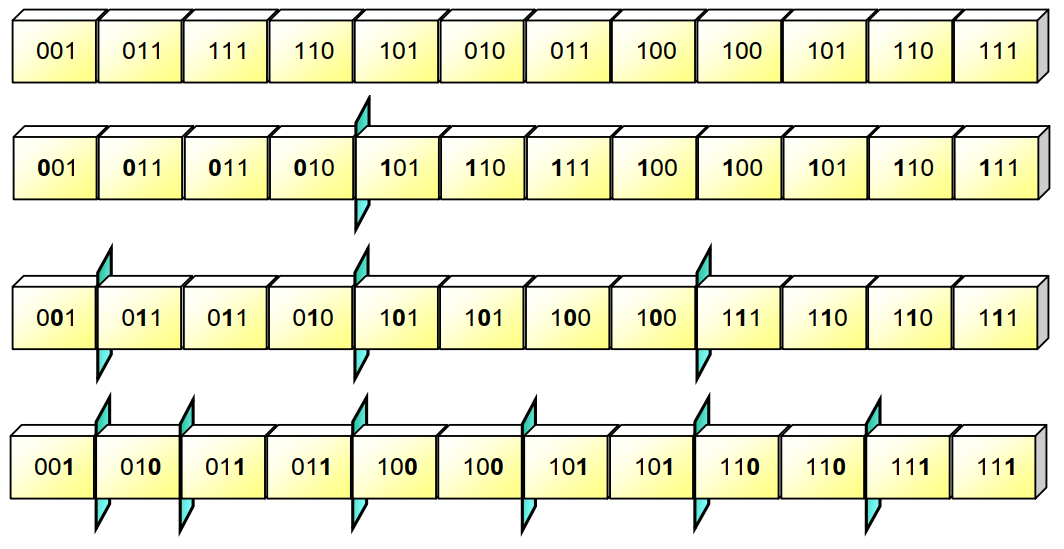
\includegraphics[scale=0.35]{sapxep/radixSort.png}

Thuật toán này chạy nhanh hơn các thuật toán khác, với độ phức tạp thời gian là $O(n.\log_k(\max(S)))$ với $\max(S)$ là phần tử lớn nhất của S, k là cơ số, ví dụ nếu chia theo từng bit, số $S_i$ có $\log_2(S_i)$ bit hay k = 2, nếu chia theo từng chữ số, thì có $\log(S_i)$ chữ số hay k = 10.

\section{Sắp xếp bằng cách đếm phân phối}
Nếu dãy S là một dãy có nhiều phần tử trùng lặp, thuật toán này sẽ hoạt động rất nhanh.

Tư tưởng của nó là ta đếm số lần xuất hiện của từng giá trị, sau đó duyệt qua các giá trị từ nhỏ tới lớn (không cần sắp xếp vì ta có thể dùng mảng để đánh dấu số lần, duyệt qua các chỉ số từ nhỏ đến lớn, nếu số lớn ta có thể nén số), thêm lần lượt các giá trị trở lại dãy.

Dễ thấy rằng ta cần duyệt qua dãy mất n thao tác, sau đó duyệt qua số lượng giá trị riêng biệt mất M thao tác, hay độ phức tạp $O(M + n)$, độ phức tạp bộ nhớ $O(M)$.
\chapter{Quy hoạch động}
\section{Giới thiệu}
Là một kỹ thuật lưu trữ các kết quả của đệ quy để sử dụng lại nhằm giảm số lần của đệ quy.

Các dạng bài toán quy hoạch rất phong phú và đa dạng, ứng dụng nhiều trong thực tế, nhưng cũng cần biết rằng, đa số các bài toán quy hoạch là không giải được, hoặc chưa giải được. Cho đến nay, người ta mới chỉ có thuật toán đơn hình giải bài toán quy hoạch tuyến tính lồi, và một vài thuật toán khác áp dụng cho các lớp bài toán cụ thể.

Cho đến nay, vẫn chưa có một định lý nào cho biết một cách chính xác những bài toán nào có thể giải quyết hiệu quả bằng quy hoạch động. Tuy nhiên để biết được bài toán có thể giải bằng quy hoạch động hay không, ta có thể tự đặt câu hỏi: "Một nghiệm tối ưu của bài toán lớn có phải là sự phối hợp các nghiệm tối ưu của các bài toán con hay không?" và "Liệu có thể nào lưu trữ được nghiệm các bài toán con dưới một hình thức nào đó để phối hợp tìm được nghiệm bài toán lớn được nghiệm bài toán lớn?"
\section{Tính số cách phân tích một số thành tổng}
Cho số tự nhiên $n\leq100$. Hãy cho biết có bao nhiêu cách phân tích số n thành tổng của dãy các số nguyên dương, các cách phân tích là hoán vị của nhau chỉ tính là một cách.

Ví dụ: n = 5 có 7 cách phân tích:
\begin{enumerate}
    \begin{multicols}{2}
        \item 5 = 1 + 1 + 1 + 1 + 1
        \item 5 = 1 + 1 + 1 + 2
        \item 5 = 1 + 1 + 3
        \item 5 = 1 + 2 + 2
        \item 5 = 1 + 4
        \item 5 = 2 + 3
        \item 5 = 5
    \end{multicols}
\end{enumerate}

Lưu ý: n = 0 vẫn coi là có 1 cách (dãy rỗng).

Ở chương quay lui ta đã giải bài toán này bằng cách liệt kê tất cả các cấu hình, bây giờ thử nghĩ xem có cách nào không cần liệt kê vẫn tính được không? Vì với n = 100 ta có tận 190,569,292 cách phân tích. Ta có nhận xét:

Nếu gọi F[m][v] là số cách phân tích v thành tổng các số nguyên dương $\leq m$. Khi đó có 2 trường hợp:
\begin{itemize}
    \item Phép phân tích không chứa số m: lúc này số cách phân tích là số cách phân tích v thành tổng các số nguyên dương $<m$, hay $\leq m-1$ và bằng F[m - 1][v].
    \item PHép phân tích có chứa ít nhất 1 số m: khi này nếu trừ m đi ở 2 vế ta được cách phân tích của số (v - m) thành tổng các số nguyên dương $\leq m$ hay F[m][v - m].
\end{itemize}

Ta thấy nếu $m>v$, rõ ràng chỉ có cách phân tích loại 1, còn nếu $m\leq v$ thì có cả 2 cách phân tích hay:
$$
F[m][v] = \left\{
    \begin{array}{cc}
        F[m-1][v] & (m > v)\cr
        F[m-1][v] + F[m][v - m] & (m \leq v)\cr
    \end{array}
\right.
$$
Đây gọi là \textbf{công thức truy hồi} thể hiện mối liên hệ giữa bài toán lớn và các bài toán con. Đáp án sẽ là F[n][n]: số cách phân tích n thành các số nguyên dương $\leq n$.

Phân tích mảng F với n = 5:

\begin{tabular}{c|cccccc}
    F & 0 & 1 & 2 & 3 & 4 & 5\cr\hline
    0 & 1 & 0 & 0 & 0 & 0 & 0\cr
    1 & 1 & 1 & 1 & 1 & 1 & 1\cr
    2 & 1 & 1 & 2 & 2 & 3 & 3\cr
    3 & 1 & 1 & 2 & 3 & 4 & 5\cr
    4 & 1 & 1 & 2 & 3 & 5 & 6\cr
    5 & 1 & 1 & 2 & 3 & 5 & 7\cr
\end{tabular}

Dễ thấy rằng F[m][v] được tính bằng phần tử cùng hàng bên trái và phần tử hàng trên, vậy suy ra trình tự tính bảng F phải là từ trái qua phải và trên xuống dưới. Vậy ta dựng giải thuật: khởi tạo dòng 0 có F[0][0] = 1 và tính bằng công thức truy hồi cho toàn bộ bảng.

\subsection{Tiết kiệm bộ nhớ và đệ quy có nhớ}
Vì nếu khởi tạo bảng F n x n trong khi ta chỉ dùng hàng trên thì gây lãng phí bộ nhớ, ta hoàn toàn có thể khởi tạo mảng chỉ có 2 hàng, tính xong hàng trên thì xuống hàng dưới, tính xong hàng dưới rồi quay lại đè lên hàng trên (ta không cần nữa), hoặc có thể tính trực tiếp trên mảng F 1 chiều n phần tử, ghi đè lên giá trị hiện tại.

Có thể thấy kĩ thuật quy hoạch động đòi hỏi phải xác định chính xác trình tự tính, vì vậy sẽ gây khó khăn trong trường hợp công thức truy hồi quá phức tạp, vì vậy người ta còn dùng đệ quy có nhớ, nghĩa là nếu chưa biết kết quả của bài toán đó thì gọi đệ quy tính, biết rồi thì ghi vào bảng F để lưu lại. Ngoài ra nó còn làm rõ hơn bản chất của đệ quy.

\section{Dãy con đơn điệu tăng dài nhất}
Cho dãy số A. Một dãy con của A là một cách chọn ra trong A một số phần tử (giữ nguyên thứ tự). Tìm dãy con đơn điệu tăng của A có nhiều phần tử nhất.

\begin{tabular}{l|l}
    INCSEQ.INP & INCSEQ.OUT\cr\hline
    11 & 8\cr
    1 2 3 8 9 4 5 6 20 9 10 &\cr
\end{tabular}

Đáp án là dãy (1, 2, 3, 4, 5, 6, 9, 10).

Nhận xét: Nếu gọi F[i] là độ dài dãy con tăng dài nhất kết thúc tại vị trí i, trong các phần tử $a[j]\leq a[i]$, ta luôn có
$$
    F[i] = \max_{1\leq j\leq i-1} F[j]+1
$$
Đây chính là công thức truy hồi, và ta đã có thể giải bài toán này trong $O(n^2)$ thay vì phải xét qua $2^n$ dãy con như phương pháp quay lui.
\subsection{Tăng tốc}
Tuy nhiên ta có thể làm tốt hơn nữa bằng cách gọi $B[k]$ là phần tử cuối cùng của dãy con tăng độ dài k. Có thể dễ dàng chứng minh rằng $B[k]\geq B[k-1]$ vì nếu $B[k]<B[k-1]$ có nghĩa là trước $F[i]$ có một $F[j]>F[i]$ mà $A[j]<A[i]$.

Vậy cách tính công thức truy hồi lần này không phải là tìm $F[j]$ lớn nhất nữa, mà là tìm $B[j]$ có $B[j]<A[i]$ và $B[j+1]>A[i]$, ta sẽ đặt lại $F[i]=j+1$ và $B[j+1]=A[i]$. Ta có thể sử dụng tìm kiếm nhị phân để tìm ra j, độ phức tạp tính toán được giảm xuống còn $O(n\log_2 n)$. Dễ nhận thấy rằng dãy B thực chất là dãy con mà ta đang tìm kiếm, và vì dãy tăng càng chậm thì dãy càng dài, đó là lí do ta đang cực tiểu hoá từng phần tử của B.

\section{Bài toán cái túi}
Có n món đồ, món thứ i có giá trị v[i] và khối lượng w[i]. Bạn có một cái túi có thể chứa W đơn vị khối lượng, hãy tìm cách chọn các món đồ sao cho giá trị thu được là lớn nhất mà không làm túi rách.

Nhận xét: Nếu gọi F[i][j] là giá trị tối đa có được nếu chọn các vật trong tập [1\dots i] và khối lượng không vượt quá j, ta có 2 khả năng khi xét tới vật i và khối lượng j:
\begin{itemize}
    \item Không lấy vật i hay giá trị thu được bằng với giá trị thu được khi xét tới vật $i-1$ với túi có thể chứa j đơn vị khối lượng. Tóm lại, $F[i][j] = F[i - 1][j]$.
    \item Lấy vật i: chúng ta mất đi w[i] đơn vị khối lượng, nhưng có thêm v[i] giá trị, hay $F[i][j] = F[i - 1][j - w[i]] + v[i]$.
    
    Lưu ý: để lấy vật i phải kèm điều kiện $j\geq w[i]$.
\end{itemize}

Và cuối cùng ta muốn giá trị thu được là tối đa nên:
$$
F[i][j] = \max(F[i - 1][j], F[i - 1][j - w[i]] + v[i])
$$

Sử dụng công thức truy hồi này cho toàn bộ các ô (i, j) có $j\geq w[i]$, với các ô còn lại (không đủ chỗ trống cho vật i) thì không thể lấy vật i, ta gán thẳng $F[i-1][j]$ cho nó.
\chapter{Các thuật toán trên đồ thị}
\section{Biểu diễn đồ thị trên máy tính}
\subsection{Ma trận kề}
Cho G = (V, E) là \textbf{đơn đồ thị} có n đỉnh 1, 2, \dots n và m cạnh. Ta có thể biểu diễn bằng một ma trận vuông cấp n với quy ước $A_{ij}=1$ hoặc true nếu có cạnh nối (i,j) và ngược lại $A_{ij}=0$ hoặc false. Nếu là đa đồ thị thì thay 1 thành số cạnh nối nó. Giá trị của $A_{ii}$ thì nên đặt theo mục đích nhưng nó thường được đật bằng 0.

Ưu điểm:
\begin{itemize}
    \item Dễ cài đặt, đơn giản, trực quan
    \item Để kiểm tra chỉ cần 1 phép so sánh
\end{itemize}
Nhược điểm:
\begin{itemize}
    \item Tốn bộ nhớ $O(n^2)$
    \item Không thể kiểm tra nhanh các đỉnh kề dẫn tới phí thời gian duyệt.
\end{itemize}
\subsection{Danh sách cạnh}
Ưu điểm:
\begin{itemize}
    \item Trong trường hợp đồ thị thưa (chẳng hạn m < 6n), nó sẽ tiết kiệm bộ nhớ vì chỉ cần 2m ô nhớ để lưu danh sách cạnh.
    \item Trong một số trường hợp khi ta phải xét tất cả các cạnh thì cài đặt danh sách cạnh sẽ làm cho việc duyệt dễ dàng hơn (thuật toán Kruskal chẳng hạn).
\end{itemize}
Nhược điểm: không thể duyệt nhanh tất cả các đỉnh kề với 1 đỉnh bất kì, ta buộc phải duyệt toàn bộ danh sách cạnh.
\subsection{Danh sách kề}
Để khắc phục yếu điểm của 2 cách biểu diễn trên, người ta đề xuất biểu diễn bằng danh sách kề. Trong danh sách này, với mỗi đỉnh v của đồ thị ta cho tương ứng với nó một danh sách gồm các đỉnh kề với nó.

Ưu điểm là dễ duyệt các đỉnh kề và các cạnh nhưng nhược điểm là khó có thể kiểm tra (u,v) là cạnh vì lúc đó ta phải duyệt toàn bộ các đỉnh kề với u.

\section{Duyệt đồ thị}
\subsection{Duyệt theo chiều sâu (Depth First Search - DFS)}
Tư tưởng của thuật toán đơn giản là, bắt đầu từ đỉnh u, ta tiếp tục duyệt các đỉnh kề với u, rồi lại tiếp tục duyệt như vậy đến khi không còn đường để đi bằng giải thuật đệ quy. Để không rơi vào vòng lặp vô tận (duyệt 1 đỉnh nhiều lần) ta đánh dấu đỉnh đó khi đi qua.

\begin{algorithmic}
    \Function{DFS}{u}
        \State $f_u\gets$ false
        \Comment{$f_v=$ true nếu đỉnh chưa thăm}
        \For{$v\in V$}
            \If{$f_v=$ true và $(u,v)\in E$}
                \State\Call{DFS}{v}
            \EndIf
        \EndFor
    \EndFunction
\end{algorithmic}

DFS trả về đường đi có thứ tự từ điển nhỏ nhất.

\subsection{Duyệt theo chiều rộng (Breadth First Search - BFS)}
Phương pháp này ưu tiên duyệt các đỉnh kề với nó hơn là tiếp tục duyệt theo chiều sâu như DFS. Với mọi đỉnh nó sẽ đẩy các đỉnh kề với nó vào danh sách chờ duyệt và duyệt theo thứ tự đến khi hết hàng chờ. Kết quả của việc này chính là duyệt theo chiều rộng.

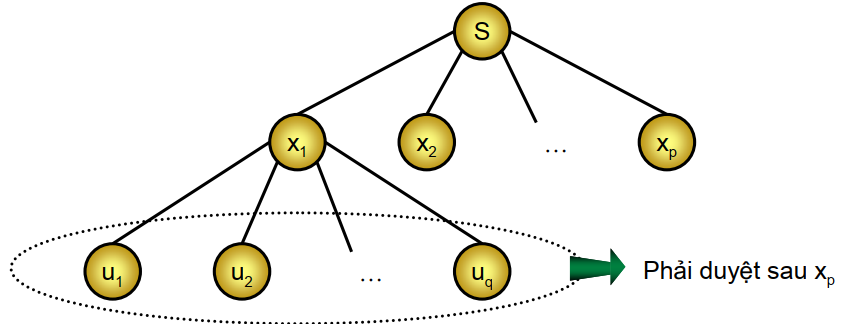
\includegraphics[scale=0.45]{dothi/bfs.png}

\begin{algorithmic}
    \Function{BFS}{}
        \State $f_s\gets$ false
        \Comment{Khởi tạo mảng đánh dấu s đã được thăm}
        \State $q\gets{s}$
        \Comment{Khởi tạo hàng đợi q chỉ chứa s}
        \While{$q\neq\emptyset$}
            \State $u\gets$\Call{Pop}{}
            \Comment{Lấy từ hàng đợi ra đỉnh u}
            \For{$v\in V$}
                \If{$f_v=$ true và $(u,v)\in E$}
                    \State $f_v=$ false
                    \State\Call{Push}{v}
                    \Comment{Đẩy v vào hàng đợi}
                \EndIf
            \EndFor
        \EndWhile
    \EndFunction
\end{algorithmic}

BFS trả về đường đi đi qua ít cạnh nhất.

\subsection{Độ phức tạp của DFS và BFS}
\begin{itemize}
    \item Trong trường hợp cài đặt bằng danh sách kề, cả hai đều có độ phức tạp $O(V+E)$, là cách cài đặt tốt nhất.
    \item Nếu biểu diễn bằng ma trận kề thì độ phức tạp là $O(n^2)$.
    \item Nếu biểu diễn bằng danh sách cạnh, việc duyệt những đỉnh kề với u sẽ phải duyệt toàn bộ danh sách cạnh, đây là cách cài đặt tồi nhất, có độ phức tạp $O(nm)$.
\end{itemize}

DFS và BFS dùng để xây dựng cây khung của đồ thị, tìm các chu trình cơ sở của đồ thị, định chiều đồ thị, liệt kê khớp-cầu của đồ thị\dots

\section{Tính liên thông. Bao đóng và thuật toán Warshall}
Với đồ thị G = (V, E) người ta xây dựng đồ thị G' = (V, E') với yêu cầu: nếu trong G u có thể đến v thì G' có cạnh nối (u,v). Lúc này G' gọi là bao đóng của đồ thị G. Dễ thấy rằng:
\begin{itemize}
    \item Một đơn đồ thị vô hướng là liên thông khi và chỉ khi bao đóng của nó là đồ thị đầy đủ.
    \item Một đơn đồ thị vô hướng có k thành phần liên thông khi và chỉ khi bao đóng của nó có k thành phần liên thông đồ thị đầy đủ.
\end{itemize}

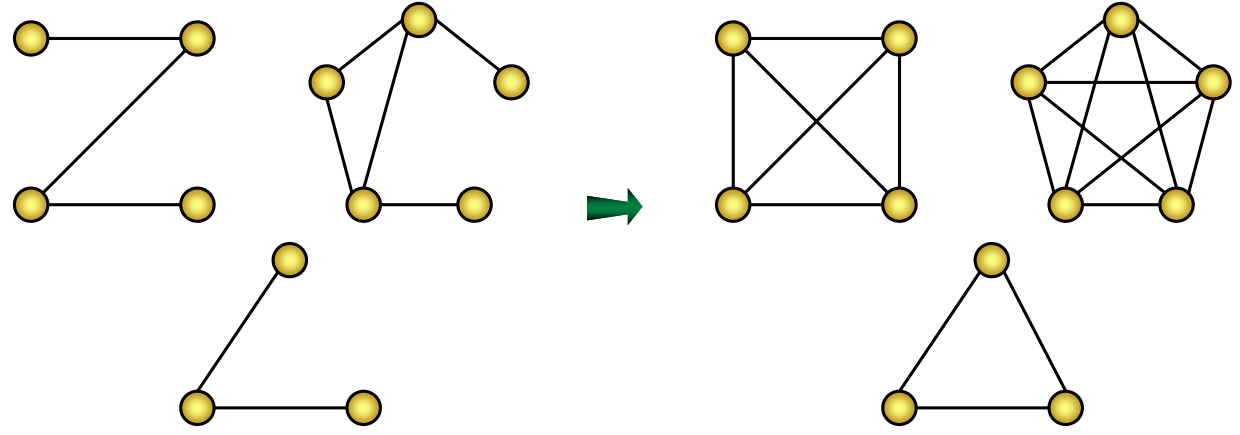
\includegraphics[scale=0.32]{dothi/baodong.png}

Thuật toán Warshall được xây dựng dựa trên định nghĩa: ta xét các cặp đỉnh (u, v): nếu có cạnh nối (u, k) và cạnh nối (k, v) thì ta nối thêm cạnh (u, v) nếu nó chưa có. Dễ thấy rằng có 3 biến chạy, độ phức tạp thời gian là $O(n^3)$.

\section{Thành phần liên thông mạnh}
Một đồ thị \textbf{có hướng} gọi là liên thông mạnh nếu như các đỉnh có thể đến được với nhau, ngược lại gọi là liên thông yếu nếu đồ thị vô hướng nền (bỏ đi các mũi tên) của nó là liên thông.

Diễn giải theo cách toán học hơn, đồ thị liên thông mạnh khi với mọi cặp đỉnh (u, v) ta có u đến được v và v đến được u, nhưng đồ thị liên thông yếu ta có u đến được v hoặc v đến được u.

\begin{figure}[h]
    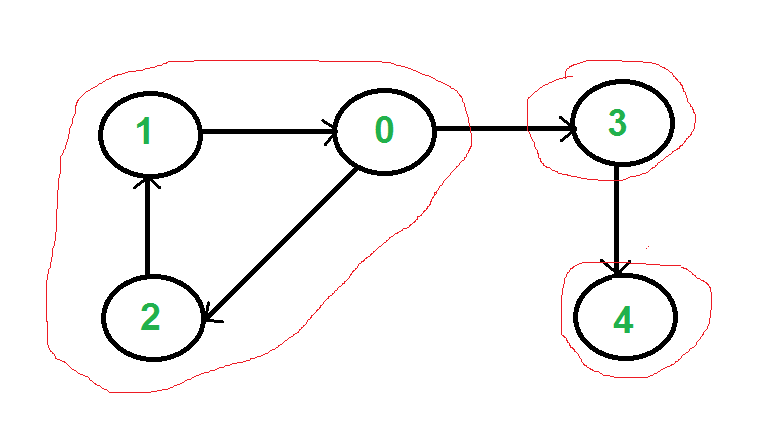
\includegraphics[scale=0.5]{dothi/ltmanh.png}
    \caption{Các thành phần liên thông mạnh}
\end{figure}

\subsection{Thuật toán Kosaraju}
Thuật toán Kosaraju xây dựng trên định nghĩa của TPLT mạnh, nó hoạt động như sau:
\begin{itemize}
    \item Sử dụng một ngăn xếp (stack) S, chọn V không thuộc S và gọi DFS(v). Đến đỉnh nào thì đẩy đỉnh đó vào S.
    \item Đảo ngược tất cả các cung.
    \item Lấy ra đỉnh trên cùng v của S. Tiếp tục gọi DFS(v). Các đỉnh có thể thăm lại được chính là các đỉnh thuộc TPLT mạnh chứa v. Ghi nhận và xoá chúng khỏi đồ thị cùng ngăn xếp S.
\end{itemize}
Cực kì đơn giản đúng không, dù độ phức tạp vẫn là O(V+E), tuy nhiên nó tốn 2 lần DFS, sẽ không hiệu quả bằng thuật toán Tarjan sắp được trình bày (chỉ tốn 1 lần DFS duy nhất), nó dựa trên rất nhiều cơ sở lí thuyết để sử dụng được.

\subsection{Một số khái niệm}
Trong cây DFS, nếu v đã được thăm trước u, có 3 khả năng xảy ra:
\begin{itemize}
    \item v là tổ tiên của u, DFS(u) do DFS(v) gọi tới. Cung (u, v) khi này gọi là \textbf{cung ngược}.
    \item v là con cháu của u, hay u đã được thăm trước v, nhưng DFS(u) sau khi đi theo hướng khác đã gọi DFS(v) rồi, nên khi đệ quy lùi lại DFS(u) sẽ thấy v là đã thăm. Lúc này cung (u, v) gọi là \textbf{cung xuôi}.
    \item v thuộc 1 nhánh cây DFS đã duyệt trước đó, hay sẽ có một đỉnh w được thăm trước cả u và v, nó rẽ sang nhánh khác thăm v trước xong rẽ sang nhánh này thăm u. Lúc này cung (u, v) gọi là \textbf{cung chéo}.
\end{itemize}
Hình bên dưới mô tả 3 cung này theo thứ tự từ trái qua phải.

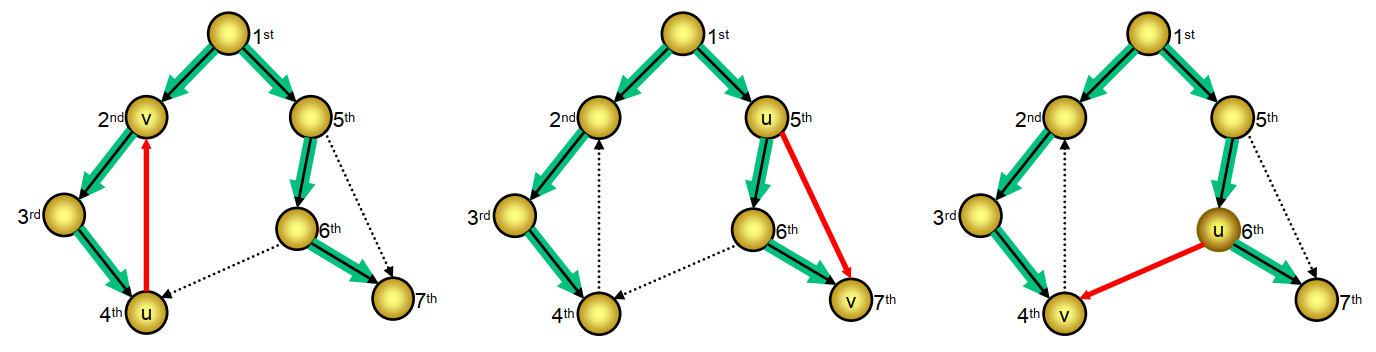
\includegraphics[scale=0.29]{dothi/cungxuoi_cungnguoc_cungcheo.png}

\subsection{Một số định lý và cơ sở lý thuyết}

\begin{theorem}
    Nếu a, b là 2 đỉnh thuộc TPLT mạnh C thì mọi đỉnh trên đường đi từ a tới b hoặc b tới a đều phải thuộc C.
\end{theorem}

Gọi v là đỉnh nằm trên đường đi từ a tới b. Nếu a muốn tới b, a phải đi qua v rồi đến b, và b muốn tới a theo con đường khác thì cũng phải đi qua v rồi mới tới a. Vậy v phải nằm trong TPLT mạnh đó.

\begin{theorem}
    Với một TPLT mạnh C bất kỳ, có một đỉnh r thuộc C sao cho mọi đỉnh của C đều thuộc nhánh DFS gốc r.
\end{theorem}

Gọi v là một đỉnh bất kỳ trong C khác r. Khi gọi DFS(r), tất cả các đỉnh kia sẽ phải thăm sau đỉnh r, rồi mới đến v. Vì v bất kỳ nên các đỉnh này phải thuộc nhánh DFS gốc r.

r còn được gọi là \textbf{chốt} của TPLT mạnh C. Trong cây DFS, chốt là đỉnh được thăm trước tất cả các đỉnh khác trong TPLT mạnh đó.

\begin{theorem}
    Nhánh DFS gốc a chỉ chứa một chốt duy nhất là a.
\end{theorem}

Với v nằm trong nhánh DFS gốc a, xét b là chốt của TPLT mạnh này. Ta sẽ chứng minh a trùng b. Nếu vậy, v cũng phải nằm trong nhánh DFS gốc b. Nếu a khác b thì có 2 khả năng:
\begin{itemize}
    \item Nhánh DFS gốc a chứa nhánh DFS gốc b, lúc này a sẽ thăm b, mâu thuẫn với giả thiết a sẽ không thăm được một chốt nào ngoài a.
    \item Nhánh DFS gốc a nằm trong nhánh DFS gốc b, hay a nằm trên đường đi từ b tới v. Theo định lý 1, a cũng phải thuộc TPLT mạnh đó, vậy nó có cả 2 chốt a và b, mâu thuẫn với khái niệm \textbf{chốt}.
\end{itemize}

Từ định lý 2 và 3 ta suy ra được: nhánh DFS gốc a chính là TPLT mạnh chứa a.

\subsection{Thuật toán Tarjan}
Chọn u là chốt mà DFS không thể tìm được chốt nào khác, ta thu được TPLT mạnh đầu tiên là nhánh DFS gốc u. Xoá nhánh này ra khỏi đồ thị, lại tìm thấy đỉnh v mà DFS không thể tìm được chốt nào khác, lại chọn TPLT mạnh thứ 2 là nhánh DFS gốc v. Tương tự với các TPLT mạnh còn lại. Có thể hình dung thuật toán này "bẻ" cây DFS tại các chốt thành các nhánh rời rạc, mỗi nhánh là một TPLT mạnh.

Nhưng cuối cùng vẫn còn một câu hỏi: Làm sao để biết v có phải chốt không? Để ý nhánh DFS gốc r.
\begin{itemize}
    \item Nếu từ các đỉnh thuộc nhánh DFS gốc r, không có cung ngược / chéo nào đi ra khỏi nhánh đó thì r là chốt. Nói cách khác, từ r chỉ có thể đến được các đỉnh thuộc nhánh DFS gốc r.
    \item Nếu từ đỉnh v của nhánh DFS gốc r có cung ngược lên đỉnh w là tổ tiên của r thì r không phải chốt.
    \item Nếu từ đỉnh v của nhánh DFS gốc r có cung chéo, ta sẽ thiết lập giải thuật sao cho khi đệ quy vừa lùi lại r, ta xoá ngay r khỏi đồ thị, vì nếu nó có chứa một chốt r' ở nhánh kia thì nó phải được duyệt rồi và bị xoá rồi, vì cung chéo sẽ chỉ đi tới nhánh thăm trước đó, chứ không đi sang nhánh thăm sau. Kể cả nếu r' là tiền bối của r thì r' phải đến được r, r có thể đến được nhánh DFS gốc r, vậy r' phải là chốt nên r không thể là chốt.
\end{itemize}

Từ 3 nhận xét trên ta rút ra được: r là chốt khi và chỉ khi không có cung nối từ một đỉnh thuộc nhánh DFS gốc r đến một đỉnh thăm trước r.

Thuật toán Tarjan xây dựng trên nhận xét này, nó đánh số cho cho các đỉnh theo thứ tự được thăm đầu tiên đến đỉnh thăm cuối cùng, gọi là \texttt{number[u]}. Ta tính thêm \texttt{low[u]} là giá trị number[\dots] nhỏ nhất trong các đỉnh đến được từ đỉnh v thuộc nhánh DFS gốc u bằng một cung (giả thiết rằng u có một cung giả nối với chính nó).

Cách tính \texttt{low[u]} như sau: Trước hết ta cho \texttt{low[u] = number[u]} hay u có cung tới chính u. Sau đó với mỗi đỉnh v nối từ u, có 2 khả năng:
\begin{itemize}
    \item Nếu v đã thăm: ta có \texttt{low[u] = min(low[u], number[v])}.
    \item Nếu v chưa thăm: ta gọi đệ quy thăm v sau đó tính \texttt{low[u] = min(low[u], low[v])}.
\end{itemize}

Dễ thấy rằng nếu \texttt{low[u] = number[u]} thì u là chốt vì không có đỉnh nào thăm trước nó.

\subsubsection{Đánh giá độ phức tạp}
Vì thuật toán Tarjan chỉ là sửa đổi một chút của thuật toán DFS bằng các thao tác O(1), nên độ phức tạp thời gian của nó bằng độ phức tạp thời gian của DFS.

\section{Bài toán đường đi ngắn nhất}
Đồ thị mà mỗi cạnh của nó được gán cho một số gọi là đồ thị có trọng số. Số gán cho mỗi cạnh gọi là trọng số của cạnh đó. Tương tự như đồ thị không trọng số thì cũng có nhiều cách biểu diễn đồ thị có trọng số trong máy tính, vd. với ma trận kề, nếu $c_{uv} = 1$ ta thay 1 thành trọng số của cạnh đó, còn nếu $c_{uv} = 0$, ta thay thành $+\infty$ hay $-\infty$, để nguyên 0\dots tuỳ thuộc vào thuật toán, sao cho dễ xử lý nhất. Quy ước $c_{vv} = 0$ với mọi v. Độ dài đường đi là tổng trọng số của các cạnh đã đi qua.

Ta sẽ chỉ xét đến đồ thị không có chu trình âm, vì nếu nó có chu trình âm (chu trình với độ dài âm), ta có thể đi qua nó vô hạn lần và mọi đường đi qua chu trình này đều sẽ có chi phí nhỏ nhất, để tránh trường hợp này người ta giải quyết bài toán \textbf{đường đi cơ bản ngắn nhất} (đường đi không có đỉnh lặp lại ngắn nhất), nhưng nó rất phức tạp.

\subsection{Thuật toán Ford - Bellman}
Có thể phát biểu cực kì đơn giản: Gọi $d_v$ là khoảng cách từ đỉnh bắt đầu s với $d_s=0$ và $d_v=+\infty\forall v\neq s$. Sau đó tối ưu hoá dần $d_v$ như sau, xét mọi cặp đỉnh u, v; nếu có bất kì cặp nào có $d_v>d_u+c_{uv}$ thì ta đặt lại $d_v=d_u+c_{uv}$. Nhớ rằng ta đặt $c_{uv}=+\infty$ nếu (u, v) không phải cung. Thuật toán kết thúc khi không thể tối ưu thêm bất kì $d_v$ nào được nữa.

\subsubsection{Tính đúng của thuật toán}
\begin{itemize}
    \item Tại bước khởi tạo thì $d_v$ là độ dài ngắn nhất từ s đến v không quá 0 cạnh.
    \item Giả sử khi bắt đầu bước i, $d_v$ bằng độ dài đường đi ngắn nhất từ s tới v không quá i - 1 cạnh, qua bước lặp nó sẽ kết nạp thêm đỉnh u vào đường đi này, vậy đường đi lúc này đã có i cạnh, suy ra được công thức trên.
    \item Sau bước lặp thứ n - 1, ta có $d_v$ là độ dài đường đi ngắn nhất không quá n - 1 cạnh, vì đồ thị không có chu trình âm nên sẽ có đường đi ngắn nhất là đường đi cơ bản (qua không quá n - 1 cạnh), vậy có không quá n - 1 bước.
\end{itemize}

Trong khi cài đặt chương trình nếu thuật toán có dạng:
\begin{minted}{cpp}
    for (int u = 1; u <= n; u++)
        for (int v = 1; v <= n; v++)
            d[v] = min(d[v], d[u] + c[u][v])
\end{minted}
Sự tối ưu bắc cầu (dùng $d_u$ tối ưu $d_v$ rồi lại dùng $d_v$ mới tối ưu $d_w$\dots) làm tốc độ tối ưu d nhanh hơn nên số bước lặp sẽ còn ít hơn nữa.

Tuy nhiên, dễ thấy rằng thuật toán có độ phức tạp $O(n^3)$. Dưới đây ta tìm hiểu các thuật toán tối ưu hơn.

\subsection{Thuật toán Dijkstra}
Nếu trọng số các cung là không âm, thuật toán Dijkstra hoạt động hiệu quả hơn so với thuật toán Ford - Bellman ở chỗ: theo công thức $d_v=\min(d_v,d_u+c_{uv})$, ta thấy $d_v$ đang được cực tiểu hoá nhờ vào $d_u$, vậy nếu sau đó $d_u$ được cực tiểu hoá thêm thì lại phải sửa lại $d_v$, dẫn tới việc phải tính đi tính lại rất nhiều lần. Vậy tại sao ta không chọn đỉnh u là đỉnh không thể cực tiểu hoá thêm nữa?

\subsubsection{Miêu tả thuật toán}
Khởi tạo như trong thuật toán Ford - Bellman, nhưng lúc này mỗi đỉnh có thêm trạng thái tự do hay cố định, nếu tự do có nghĩa là khoảng cách từ s tới nó có thể tối ưu được thêm nữa, ngược lại với cố định. Ta sẽ đánh dấu bằng mảng Free[v]. Ban đầu các đỉnh đều tự do.

Bắt đầu bước lặp, chọn trong các đỉnh đang tự do, lấy ra đỉnh u có $d_u$ nhỏ nhất và cố định nó. Dùng đỉnh này tối ưu hoá tất cả các đỉnh v khác theo công thức tối ưu đỉnh như trên. Bước này sẽ kết thúc khi đỉnh f bị cố định, hoặc tất cả các đỉnh tự do đều không có đường đi tới nó.

Nếu vậy, tại sao ở thao tác 1, $d_u$ lại được cố định, lỡ có đỉnh t sao cho $d_u>d_t+c_{tu}$ thì sao, do trọng số $c_{tu}$ không âm, nên $d_u>d_t$, mâu thuẫn với giả thiết $d_u$ nhỏ nhất. Trong lần lặp đầu tiên s là đỉnh được cố định đầu tiên với $d_s=0$.

Cuối cùng thông báo đường đi ngắn nhất, lưu vết trong khi tính hoặc thông báo không có đường đi tới đỉnh đó.

\subsubsection{Tối ưu bằng heap}
Nếu đồ thị thưa (nhiều đỉnh, ít cạnh) có thể dùng danh sách kề kèm trọng số để biểu diễn nhưng thời gian tìm đỉnh có khoảng cách ngắn nhất vẫn là $O(n)$, hay độ phức tạp của thuật toán Dijkstra là $O(n^2)$. Để tối ưu nó, người ta dùng heap với quy tắc nếu v là con của u thì $d_v\geq d_u$, vậy đỉnh ở gốc heap là đỉnh có khoảng cách nhỏ nhất, giống với min heap. Tại bước lặp ta sửa lại như sau: Thao tác tìm đỉnh cố định sẽ lấy đỉnh lưu ở gốc heap, đưa phần tử cuối heap vào thế chỗ và vun đống. Vì thao tác vun đống có độ phức tạp $O(\log_2 n)$ (duyệt theo chiều cao của cây), vậy ta đã tối ưu thao tác tìm đỉnh từ $O(n)$ xuống $O(\log_2 n)$, hay độ phức tạp của thuật toán Dijkstra lúc này là $O(\max(n,m)\log_2 n)$.

\subsection{Sắp xếp tô-pô}
Cơ sở của thuật toán là: nếu G = (V, E) là một đồ thị có hướng không chu trình (Directed Acyclic Graph - DAG), các đỉnh của nó có thể đánh số sao cho mỗi cung của G nối từ đỉnh có bán bậc vào nhỏ hơn đến đỉnh có bán bậc vào lớn hơn. Tiếp tục dùng đoạn code:
\begin{minted}{cpp}
    for (int u = 1; u <= n; u++)
        for (int v = 1; v <= n; v++)
            d[v] = min(d[v], d[u] + c[u][v])
\end{minted}
Hãy tưởng tượng: ta bắt đầu bằng một đỉnh không có cung đi vào (bán bậc vào bằng 0, vì nếu mọi đỉnh đều có bán bậc vào, thì nó có chu trình), chắc chắn đường đi của nó không thể tối ưu thêm, vậy ta dùng đỉnh này tối ưu các đỉnh khác, sau đó xoá đỉnh này ra khỏi đồ thị cùng những cung đi từ nó, ta lại được một DAG mới cũng không có chu trình, tiếp tục làm như vậy đến khi xoá tất cả các đỉnh khỏi đồ thị. Một lần nữa, độ phức tạp thời gian của thuật toán là $O(n^2)$, tuy nhiên nếu dùng danh sách kề thì độ phức tạp của nó chỉ còn là $O(m)$.

\subsection{Thuật toán Floyd}
Bài toán đặt ra lúc này là tính tất cả d(u, v) là khoảng cách từ u tới v. Thay vì dùng các thuật toán 1 đỉnh xuất phát như trên, ta có thể tối ưu hoá dần ma trận trọng số theo công thức \texttt{c[u][v] = min(c[u][v], c[u][k] + c[k][v])}.

\subsubsection{Tính đúng của thuật toán}
Gọi $c^k[u][v]$ là độ dài đường đi ngắn nhất từ u tới v qua các đỉnh trung gian thuộc tập \{1\dots k\}. Khi k = 0 thì $c[u][v]=c^0[u][v]$ (đường đi ngắn nhất là đường đi trực tiếp).

Giả sử đã tính được $c^{k-1}[u][v]$ thì ta tính $c^k[u][v]$ như sau: Nếu đường đi ngắn nhất từ u tới v mà chỉ qua các đỉnh trong tập \{1\dots k\} thì:
\begin{itemize}
    \item Nếu không qua đỉnh k, thì nó chỉ đi qua các đỉnh trong tập \{1\dots k-1\}, hay $c^k[u][v]=c^{k-1}[u][v]$.
    \item Nếu có đi qua đỉnh k thì đó là đường đi từ u đến k nối với đường đi từ k đến v, 2 đường đi này chỉ đi qua các đỉnh thuộc tập \{1\dots k-1\} hay $c^k[u][v]=c^{k-1}[u][k]+c^{k-1}[k][v]$.
\end{itemize}
Vì ta muốn $c^k[u][v]$ cực tiểu nên ta có
$$c^k[u][v] = \min(c^{k-1}[u][v], c^{k-1}[u][k] + c^{k-1}[k][v])$$

Lúc này ta quan tâm tới $c^n[u][v]$ là độ dài đường đi ngắn nhất từ u tới v qua n đỉnh. Khi cài đặt ta sẽ không chia theo biến k nhưng sẽ thao tác trực tiếp trên mảng c, sự tối ưu bắc cầu sẽ tăng tốc độ tối ưu cho các đỉnh. Lại như thuật toán Ford-Bellman, nó có 3 biến chạy, vì vậy ta dùng 3 vòng lặp lồng nhau, hay độ phức tạp tính toán $O(n^3)$.

\section{Bài toán cây khung nhỏ nhất}
\subsection{Thuật toán Kruskal}
Với đồ thị G = (V, E) có n đỉnh, khởi tạo cây T không có cạnh nào. Xét tất cả các cạnh của đồ thị từ trọng số nhỏ tới lớn, nếu việc thêm cạnh đó vào T không tạo thành chu trình đơn trong T thì thêm cạnh đó vào T. Thuật toán kết thúc khi đã thêm đủ n - 1 cạnh (thành công), hoặc nếu thêm cạnh nào cũng tạo thành chu trình đơn trong T thì thông báo tìm kiếm cây khung thất bại.

\textbf{Chú ý:}
\begin{itemize}
    \item Ta có thể dùng thuật toán Heap Sort cho hiệu quả vì mỗi lần vun đống ta mất $O(\log n)$, nhưng hiếm khi nào ta phải duyệt toàn bộ danh sách cạnh, nên thay vì sắp xếp toàn bộ sẽ mất $O(n\log n)$, chắc chắn ta đạt được độ phức tạp nhỏ hơn con số đó.
    \item Muốn thêm một cạnh (u, v) vào T mà không tạo thành chu trình đơn thì nó phải nối 2 cây khác nhau của T, kiểm tra bằng cách kiểm tra gốc của chúng.
    \item Khi cài đặt, để kiểm tra gốc của chúng ta dùng một mảng Lab với Lab[v] là gốc của cây chứa v. Ngoài ra để tránh cây bị suy biến ta có thể coi một cây là con của cây khác, với quy ước cây nào ít nút hơn sẽ là con của cây kia.
\end{itemize}

\subsection{Thuật toán Prim}
Nếu đồ thị dày thì thuật toán Kruskal sẽ hoạt động chậm, lúc này người ta sẽ dùng thuật toán Prim. Nó được phát biểu như sau:

Đơn đồ thị vô hướng G = (V, E) được cho bởi ma trận trọng số C. Quy ước $c_{uv}=+\infty$ nếu (u, v) không là cạnh. Xét cây T và 1 đỉnh v, gọi $d_{uv}$ (khoảng cách từ v tới T) là trọng số nhỏ nhất trong các cạnh nối v với đỉnh nào đó trong T. Ban đầu cây T chỉ có đỉnh 1. Sau đó cứ chọn trong số các đỉnh ngoài T ra 1 đỉnh gần T nhất, thêm đỉnh đó và cạnh nối đỉnh đó với T vào T luôn đến khi đã đủ n đỉnh hoặc chưa đủ nhưng mọi đỉnh ngoài T đều có khoảng cách $+\infty$. Khi này đồ thị không liên thông, tìm kiếm cây khung thất bại.

Nhìn chung thuật toán hoạt động giống như thuật toán Dijkstra, nên cũng có độ phức tạp $O(n^2)$, có thể dùng heap để tối ưu trở thành $O(\max(n,m)\log_2n)$, tuy nhiên nếu làm việc với đồ thị thưa người ta dùng thuật toán Kruskal chứ không dùng thuật toán Prim với heap.

\end{document}